\subsection{A very basic introduction to networking}
Let's say we have an office in NY. In that office there are end-hosts, such as PCs, server, printers, etc. All of the end hosts need to communicate with each other, for this we introduce a switch, this switch is going to be connected to each of the end-hosts using ethernet cables. A switch is a device with a lot of ports - which are basically slots to connect ethernet cables to - this allows the device to be connected to each other through the switch. The switch is what allows connectivity on my \emph{local area network}. Let's say we add another end-host, a laptop, which is connected wirelessly to the same switch, the laptop will be connected via WIFI to a \emph{wireless access point} and the wireless access point is connected to the switch via an ethernet cable. Now that all the end-hosts are able to communicate, we have built a \emph{local area network}, which means a network that connects devices within the same local area, such as an office or a university campus.


Now that we have built a local area network, we also want these end-hosts to be able to communicate with other devices out on the internet, not just in my local area network. For this we introduce another component, the \emph{router}, which is a device capable of making advanced routing decisions to route traffic between different areas of your network.


Next, now that we have connected the end-hosts to the local are network, and the local area network to the internet via a router. The internet is a very dangerous place, hackers can attack us and other things that we don't want can happen. For security reasons we install a \emph{firewall}, which secures the different parts of our network from each other.


In a larger company we would not just have end-hosts connected to switches connected to routers connected to firewalls connected to the internet. We would have similar local area networks in many other places, for example, we can say that we have a very similar local area network in Boston. The same devices and the same connections. Lets say we want the NY and Boston office to communicate directly without using the internet. We can use a \emph{dedicated connection} between my two routers on both sites for communications to be direct from the NY router to the Boston router, this is called a \emph{wide area network}.


All this is expressed in the next, \emph{network topology diagram}.
\begin{figure}[H]
    \centering
    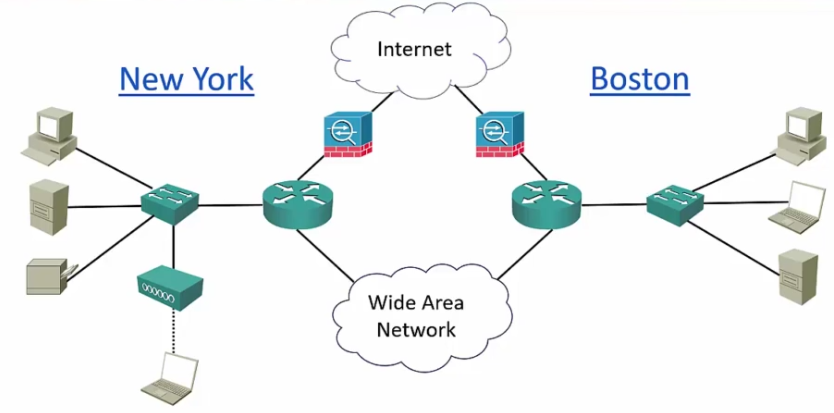
\includegraphics[width=\width\textwidth]{./figs/2021-10-10-13-28-12.png}
    % 	\caption{}
\end{figure}

Some other caracteristics of networks are:
\begin{itemize}
    \item Topology: how the devices are connected to the each other.
    \item Speed: the faster, the more cost.
    \item Cost: the monetary cost, effected by the type of devices and technologies used.
    \item Security: all the security features inside and outside the devices.
    \item Availability: making sure that our network always stays up. Mission critical components are typically duplicated, that way we can have an alternative if one were to fail.
    \item Scalability: the topology design lends itself to grow as needed.
    \item Reliability: similar to availability, making sure the network is going to continue to work.
\end{itemize}

%----------------------------------------------------------------------------------------
\section{The OSI Reference model}
\begin{itemize}
    \item The OSI model stands for Open Systems Interconnect model. 
    \item It is standardized by the Organization for Standardization (ISO).
    \item It is a general purpose network that standardizes how computers communicate with one another over a network.
    \item The OSI model is conceptual it is not a physical thing, device, or protocol. It is a concept for humans only, to be able to understand. 
    \item The 7 layer approach to data transmission divides the operations into specific related groups of actions at each layer. A layer serves the layer above it and is served by the layer below it.
\end{itemize}
\subsection{Example}
An example is how you send an email. The sender (the person sending the email) and the receiver (the person receiving the email). 
In the layer 7 - the application layer - which is the layer containing the ``from:'' or the ``to:'' field, this is collected at an application layer. Next the data will be encapsulated by the layer 6 - presentation layer - which deals with the format the data is being handled with. Then the layer 6 information is encapsulated into the layer 5 - session layer - information. That then gets encapsulated to the 4th layer - the transport layer -  which is the layer that specifies what communcation will be used - TCP, UDP, Port number - to prepare it for the next layer. That gets encapsulated into layer 3 - the network layer - which includes the source and destination IP address, a device that operates at layer 3 is the routers. The next the packet is almost being finished, and passed on to the layer 2 - the data link layer - which specifies the mac address - in case we are sending this over an ethernet network -, devices that operate at this layer are switches. Finally the encapsulated and consolidated packet is ready to be sent, this is done in layer 1 - which is the Physical layer - which literally means sending the packet through the wire, a network device that used to be used in this layer are hubs - which are not used anymore -. The email has been sent. The packets travel through the wires and devices to the receiver and the receiver receives packets in the form of electrical signals. 
\begin{figure}[H]
    \centering
    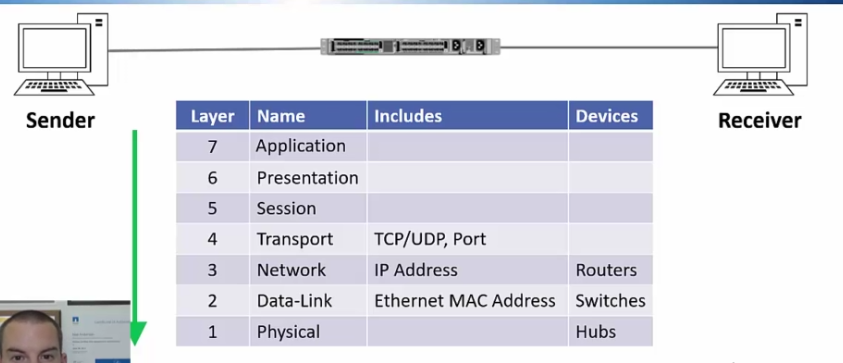
\includegraphics[width=\width\textwidth]{./figs/2021-10-10-13-54-03.png}
% 	\caption{}
\end{figure}
The receiver will process the information being received from layer 1 to layer 7, which means that the receiver will grab the data from the first layer and decapsulate it until it has layer 7 data. It comes in at the physical layer, then it it will pass to the data link layer which is 2nd layer, it will perform checks to ensure that the the destination mac address is really for the receiver, if it is not, the receiver will just discard the packet. Next it will look at the layer 3 - which is the network layer - it will check the destination ip address and check if the packet is for it, otherwise it will discard the packet. Then we carry on with the next layer, layer 4 - the transport layer - it will check the port number in which it was received and some other validations. It will continue through the session layer - layer 5 -, the presentation layer - layer 6 -, and the application layer - layer 7 -.
\begin{figure}[H]
    \centering
    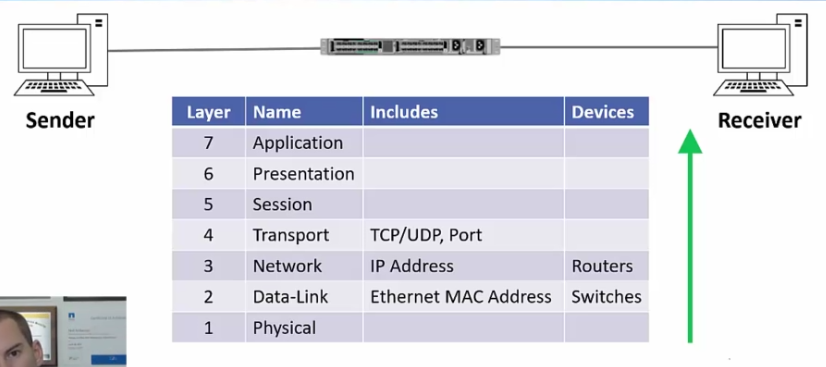
\includegraphics[width=\width\textwidth]{./figs/2021-10-10-14-12-16.png}
% 	\caption{}
\end{figure}
Layer 6 and 7 - application and presentation - are considered the upper level, typically used by developers not network engineers. Usually network engineers start to become interested from layer 4 downward.

\subsection{Benefits of the OSI model}
\begin{itemize}
    \item Engineers don't need to design technologies to work end to end from top to bottom of the model. Instead they can just focus on their layer of expertise, and make sure they comply with the standards for the layers above and below.
    \item This leads to open standards and multi-vendor interoperability. 
    \item For example: if you're an application developer, you can just focus on the top three layers, the lower layers are the domain of network engineers. You don't need to understand thzem, you just make sure you are complying with the standards.
    \item Troubleshooting is easier because you can analyse a problem in a logical fashion layer by layer.
    \item It is difficult to convey how important the OSI model is. The OSI model is used to describe problems, solutions, technologies, etcetera. Such as if the cable was disconnected you would say 'it was a layer 1 problem', if you find that the problem was that the user specified a wrong destination - you say - 'it was a layer 7 problem, etcetera.
\end{itemize}

\subsection{OSI Acronyms}
\begin{itemize}
    \item The classic: Please Do Not Throw Sausage Pizza Away.
    \item Network Relevant: Please Don't Need Those Stupid Packets Anyway.
    \item Us relevant: Please Do Not Teach Students Pointless Acronyms.
    \item Useful: Please Do Not Take Sales People's Advice.
    \item Favorite: Please Do Not Touch Superman's Private Area.
\end{itemize}


\section{TCP/IP Stack}
\begin{itemize}
    \item TCP/IP was developed during the 1960s by the US department of defense's Advanced Research Projects Agency (ARPA).
    \item It is a protocol stack which consists of multiple protocols including TCP (Transmission Control Protocol) and IP (Internet Protocol). It is not a single protocol, it is a protocol stack.
    \item An analogy to understand what a protocol is is when diplomats meet each other, there is a certain way they are expected to behave and to communicate with each other, in computer networking protocols basically mean the same thing. You have two hosts and they are going to communicate with each other, there has to be a protocol that describes that communication is going to be and how is it going to behave.
    \item It is the main protocol stack used in computer operations today.
        \begin{itemize}
            \item There used to be many other protocols such as Ipxspx and apple talk. But today TCP/IP is pretty much standard, other protocols are pretty much dead.
        \end{itemize}
    \item Whereas the OSI reference model is conceptual, the TCP/IP stack is actually used to transfer data in production networks.
    \item TCP/IP is also layered but does not use all the OSI layers, though the layers are equivalent in operation and function.
        \begin{itemize}
            \item It does actually use all of the layers, but in the documentations only 4 are layed out.
        \end{itemize}
\end{itemize}

%----------------------------------------------------------------------------------------
\subsection{Comparing the OSI model with the TCP/IP}

\begin{figure}[H]
    \centering
    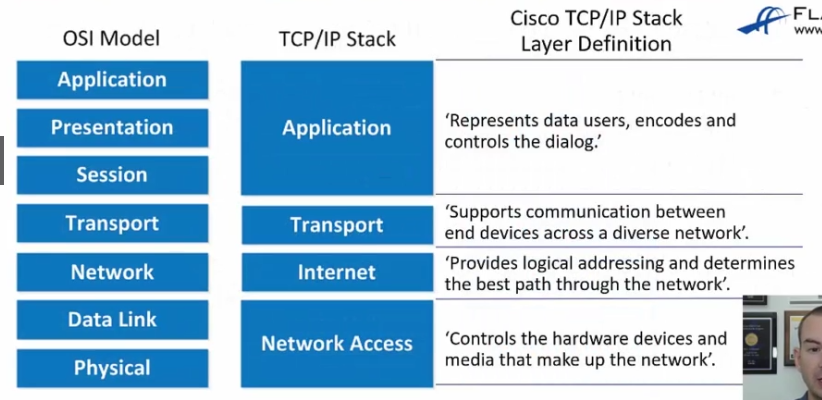
\includegraphics[width=\width\textwidth]{./figs/2021-10-10-20-20-19.png}
% 	\caption{}
\end{figure}
Notice that the TCP/IP does cover all the layers of the OSI model, however it sometimes uses the layers together. The application layer - in the TCP/IP - maps to the OSI model's layer 5,6, and 7 - session, presentation, and application -.
Below that we have the transport layer - in the TCP/IP stack - which notice maps directly to the transport layer in the OSI model. The internet layer in the TCP/IP is equivalent to the network layer in the OSI model. Last we have the network access in the TCP/IP stack that maps to the OSI layer 1 and 2 - physical and data-link-.

\begin{itemize}
    \item While both the OSI model and the TCP/IP stack are very important in networking. We are going to typically be referencing more the OSI model than the TCP/IP stack.
\end{itemize}

\subsection{Hosts communication terminology}
When two hosts communicate with each other, they talk using something called protocol data unit (PDU), which is the entire communication that happens on the OSI model (sender from layer 7 to layer 1 and receiver from layer 1 back to layer 7).

The data exchanged varies in terminology according to which layer of the TCP/IP stack is being talked about.
\begin{itemize}
    \item The application layer communicates using data to the application layer in the other host.
    \item The transport layer communicates using segments to the transport layer in the other host.
    \item The internet layer communicates using packets to the internet layer in the other host.
    \item The network access layer communicates using frames to the network access layer of the other host.
\end{itemize}
\begin{figure}[H]
    \centering
    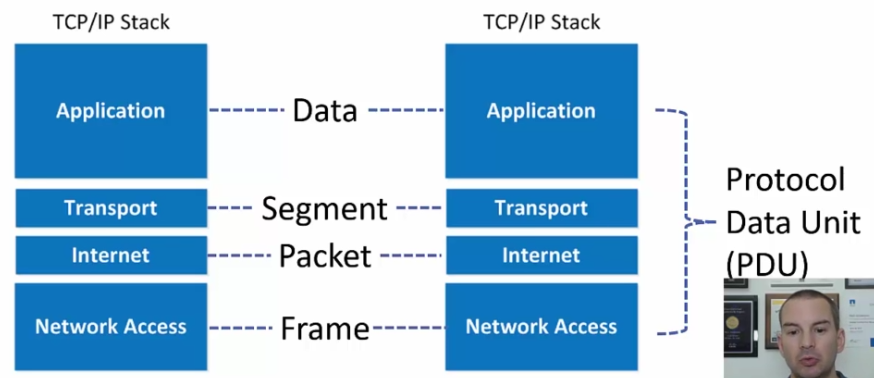
\includegraphics[width=\width\textwidth]{./figs/2021-10-10-20-30-40.png}
% 	\caption{}
\end{figure}
In the networking world the OSI model is more commonly referenced than the TCP/IP stack in terms of layers - which means that it is more common to refer to the layers of the OSI model than the layers of the TCP/IP -. However when we are talking about host communications terminology, it is more common to speak of the TCP/IP communications terminology - which means that it is more common to use 'data' if you are refering to the layer 5,6, and 7 of the OSI model, layer 3 call it a packet, layer 4 call it a segment-. Another very important thing is that networking people usually refer to the PDU as the name packet, the correct name is a PDU not a packet since the packet is used for layer 2 (internet layer) communication, but people typically use the term packet and PDU interchangeably, while technically wrong, but in day-to-day communcations when refering to host communications it is not uncommon to call it packet meaning the entire stack.


%----------------------------------------------------------------------------------------
\section{The upper OSI layers}
\begin{itemize}
    \item The networking engineers do not typically work directly with the upper 3 layers of the OSI model, but we still need to know what they do.
    \item They are more relevant to application developers.
    \item In this lecture I will primarily be giving you the Cisco definitions of the layers.
    \item Information included in the upper layers would include the message body and subject line in an email message for example.
\end{itemize}

\subsection{Layer 7 - the application layer}
\begin{itemize}
    \item The application layer provides network services to the applications of the end user.
    \item If differs from the other layers in that it does not provide services to any other OSI layer.
    \item The application layer establishes the availability of intended communications partners.
        \begin{itemize}
            \item Intended communcation partners are the hosts that the current hosts is trying to communicate with.
        \end{itemize}
    \item It then synchronizes and establishes agreement on procedures for error recovery and control of data integrity.
        \begin{itemize}
            \item Data integrity is verifying that data has not been corrupted or damaged in transit.
        \end{itemize}
\end{itemize}

\subsection{Layer 6 - the presentation layer}
\begin{itemize}
    \item The presentation layer ensures that the information that is sent at the application layer of one system is readable by the application layer of another system.
    \item The presentation layer can translate among multiple data formats using a common format (eg computers with different encoding schemes)
\end{itemize}

\subsection{Layer 5 - session layer}
\begin{itemize}
    \item The session layer establishes, manages, and terminates sessions between two communicating hosts.
    \item THe session layer also synchronizes dialog between the presentation layers of the two hosts and manages their data exchange.
    \item For example, web servers have many users, so there are many communication processes open (session) at anygiven time to track. The session layer keeps track of all of the opened sessions.
    \item It also offers efficient data transfers, CoS (Class of Service), and exception reporting of upper layer problems.
\end{itemize}


%----------------------------------------------------------------------------------------
\section{The lower OSI layers}
\begin{itemize}
    \item Whereas network engineers are not particularly interested in the upper OSI layers, we are very concerned with the lower 4 layers of the OSI model. These are incredibly important and are almost like the daily routine to network engineer.
    \item Each of these layers have their own dedicated section later and you will learn much more detailed information about them throughout the course.
\end{itemize}

\subsection{Layer 4 - transport layer}
\begin{itemize}
    \item The main characteristics of the transport layer are wether TCP or UDP transport is used, and the port number. 
    \item We haven't really seen what is TCP and UDP, for now you can think of it as modes of transportation where each one has different advantages. The TCP is very reliable, therefore if priority is reliability we use TCP. If speed is more important than reliability - like for voice of video traffic - then we use UDP instead.
    \item We haven't seen what ports are, but for now you just need to know that different processes occur in these ports, for example the 80th port is used for http web traffic and port 25 is used for email.
    \item Definition:
        \begin{itemize}
            \item The transport layer defines services to segment, transfer, and reassemble the data for individual communications between the end devices.
            \item It breaks down large files into smaller segments that are less likely to incur transmission problems.
        \end{itemize}
\end{itemize}

\subsection{Layer 3 - network layer}
\begin{itemize}
    \item The most important information at the network layer is the source and destination IP address. Other information is also carried, but the main is the source and destination of IPs.
    \item Routers operate at layer 3.
    \item Definition: 
        \begin{itemize}
            \item The network layer provides connectivity and path selection between two host systems that may be located on geographically separated networks. 
            \item The network layer is the layer that manages the connectivity of hosts by providing logical addressing (IP addressing is our logical addressing).
        \end{itemize}
\end{itemize}

\subsection{Layer 3 - the data-link layer}
\begin{itemize}
    \item The most important information at the data-link layer is the source and destination layer 2 address. Again - just like in layer 3 and 4 - there is also other information but the main one is the source and destination layer address.
    \item For example the source and destination MAC address if ethernet is the layer 2 technology. Different layer 2 technologies use different formats for their addressing, for example, old legacy frame relay uses DLCI or DCE numbers for the addressing. Today the typical address used at this layer is the MAC address.
    \item Switches operate at layer 2.
    \item Definition:
        \begin{itemize}
            \item The data link layer defines how data is formated for transmission and how access to physical media is controlled.
            \item It also typically includes error detection and correction to ensure a reliable delivery of data.
        \end{itemize}
\end{itemize}

\subsection{Layer 1 - the physical layer}
\begin{itemize}
    \item The physical layer concerns literally the physical components of the network, for example the cables being used.
    \item Definition:
        \begin{itemize}
            \item The physical link enables bit transmission between end devices.
            \item It defines specifications needed for activating, maintaining, and deactivating the physical link between end devices.
            \item For example, voltage levels, physical data rates, maximum transmission distances, physical connectors, etcetera.
        \end{itemize}
\end{itemize}
